% $Id$
% Author:  Daniel Bosk <daniel.bosk@miun.se>
\documentclass{beamer}
\usepackage[utf8]{inputenc}
\usepackage[T1]{fontenc}
\usepackage[english,swedish]{babel}
\usepackage{url}
\usepackage{varioref,prettyref}
\usepackage{graphicx}
\usepackage[today,nofancy]{svninfo}
\usepackage{natbib}
\usepackage{booktabs}
\usepackage[varioref,prettyref]{miunmisc}
\setcitestyle{numbers,square}
\bibliographystyle{swealpha}

\renewcommand{\qedsymbol}{Q.E.D.}
\newcommand{\N}{\mathbb{N}}
\newcommand{\Q}{\mathbb{Q}}
\newcommand{\R}{\mathbb{R}}
\newcommand{\Z}{\mathbb{Z}}
\newcommand{\powerset}{\mathcal{P}}
\newcommand{\U}{\mathcal{U}}
\newcommand{\V}{\mathcal{V}}
\DeclareMathOperator{\card}{card}
\DeclareMathOperator{\tnot}{icke}
\DeclareMathOperator{\tor}{eller}
\DeclareMathOperator{\tand}{och}
\DeclareMathOperator{\lequiv}{\Longleftrightarrow}
\DeclareMathOperator{\congruent}{\equiv}
\DeclareMathOperator{\xor}{\oplus}

\providetranslation[to=swedish]{Theorem}{Sats}
\providetranslation[to=swedish]{Corollary}{Korollarium}
\theoremstyle{definition}
\newenvironment{axiom}[1]{\begin{block}{Postulat (#1)}}{\end{block}}
\providetranslation[to=swedish]{Example}{Exempel}
\newtheorem{exercise}{Övning}
\theoremstyle{remark}
\newtheorem{remark}{Anmärkning}

\svnInfo $Id$

\mode<presentation>
{
  \usetheme{Frankfurt}
  \setbeamercovered{transparent}
  \usecolortheme{seagull}
}
\setbeamertemplate{footline}{\insertframenumber}

\title{%
  Datarepresentation
}
\author{Daniel Bosk\footnote{%
  \tiny
  Detta verk är tillgängliggjort under licensen Creative Commons 
  Erkännande-DelaLika 2.5 Sverige (CC BY-SA 2.5 SE).
  För att se en sammanfattning och kopia av licenstexten besök URL 
  \url{http://creativecommons.org/licenses/by-sa/2.5/se/}.
}}
\institute[MIUN IKS]{%
  %Department of Information and Communication Systems (ICS),\\
  %Mid Sweden University, Sundsvall.
  %
  Avdelningen för informations- och kommunikationssytem (IKS),\\
  Mittuniversitetet, Sundsvall.
}
\date{\svnId}

\pgfdeclareimage[height=0.65cm]{university-logo}{MU_logotyp_int_CMYK.pdf}
\logo{\pgfuseimage{university-logo}}

\AtBeginSection[]{%
  \begin{frame}<beamer>{Översikt}
    \tableofcontents[currentsection]
  \end{frame}
}

\begin{document}

\begin{frame}
  \titlepage
\end{frame}

\begin{frame}{Översikt}
  \tableofcontents
  % You might wish to add the option [pausesections]
\end{frame}

\begin{frame}
  Innan du påbörjar laborationen ska du ha läst kapitel 1, 2, 5 och 6.1--6.4 
i \cite{Brookshear2012csa} och avsnitt 2--4 i \cite{pythonkramaren1}.

\end{frame}


% Since this a solution template for a generic talk, very little can
% be said about how it should be structured. However, the talk length
% of between 15min and 45min and the theme suggest that you stick to
% the following rules:  

% - Exactly two or three sections (other than the summary).
% - At *most* three subsections per section.
% - Talk about 30s to 2min per frame. So there should be between about
%   15 and 30 frames, all told.


\section{Talsystem}

\subsection{Olika talsystem}

\begin{frame}{\insertsubsectionhead}
  \begin{table}
    \caption{Olika representationer av etthundratjugotre i olika talsystem.}
    \begin{tabular}{ll}
      \toprule
      Binära talsystemet & \(1111011\) \\
      Decimala talsystemet & \(123\) \\
      Hexadecimala talsystemet & \(7B\) \\
      Romerska talsystemet & CXXIII \\
      \bottomrule
    \end{tabular}
    \label{tbl:OlikaEtthundratjugotre}
  \end{table}
\end{frame}

\begin{frame}{\insertsubsectionhead}
  \begin{figure}
    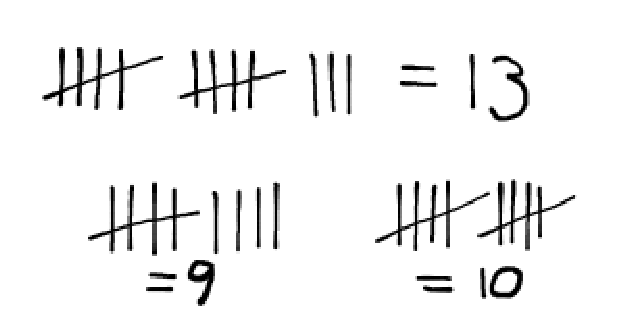
\includegraphics[width=4cm]{strecktal.eps}
    \caption{Tecknen i ett enkelt teckenvärdessystem.}
    \label{fig:Strecktal}
  \end{figure}
\end{frame}

\begin{frame}{\insertsubsectionhead}
  \begin{table}
    \caption{De romerska siffrorna.}
    \begin{tabular}{ccccccc}
      \toprule
      I & V & X & L & C & D & M \\
      1 & 5 & 10 & 50 & 100 & 500 & 1000 \\
      \bottomrule
    \end{tabular}
    \label{tbl:RomerskaSiffror}
  \end{table}
\end{frame}

\begin{frame}{\insertsubsectionhead}
  \begin{table}
    \caption{Talen 1-10 i det decimala och det romerska talsystemen.}
    \begin{tabular}{l|llllllllll}
      \toprule
      Decimala talsystemet & 1 & 2 & 3 & 4 & 5 & 6 & 7 & 8 & 9 & 10 \\
      Romerska talsystemt & I & II & III & IV & V &
        VI & VII & VIII & IX & X \\
      \bottomrule
    \end{tabular}
    \label{tbl:RomerskaTal}
  \end{table}
\end{frame}

\begin{frame}{\insertsubsectionhead}
  \begin{table}
    \caption{Några tal skrivna med det romerska talsystemet.}
    \small
    \begin{tabular}{lll}
      \toprule
      \(2011\) & MMXI & \(1000+1000+10+1\) \\
      \(1999\) & MCMXCIX & \(1000+(1000-100)+(100-10)+(10-1)\) \\
      \(1998\) & MCMXCVIII & \(1000+(1000-100)+(100-10)+5+1+1+1\) \\
      \(587\) & DLXXXVII & \(500+50+10+10+10+5+1+1\) \\
      \(487\) & CDLXXXVII & \((500-100)+50+10+10+10+5+1+1\) \\
      \bottomrule
    \end{tabular}
    \label{tbl:RomerskaTal2}
  \end{table}
\end{frame}


\subsection{Positionssystem}

\begin{frame}{\insertsubsectionhead}
  \begin{example}\label{ex:PositionensBetydelse}
    I \(111\) betyder den första ettan \(100\) medan den andra ettan
    betyder \(10\) och den sista betyder \(1\).
    Det vill säga, samma siffra har olika betydelse beroende på vilken position
    den har i representationen som den befinner sig i.
  \end{example}
\end{frame}

\begin{frame}{\insertsubsectionhead}
  \begin{example}\label{ex:DecimaltPosistionssystem}
    Det decimala talsystemet har basen \(10\).
    Talet etthundratjugotre representeras i detta system som \(123\).
    Vi har då
    \[1\cdot10^2 + 2\cdot10^1 + 3\cdot10^0 = 100 + 20 + 3 = 123.\]
  \end{example}

  \begin{example}\label{ex:BinartPositionssystem}
    Det binära talsystemet har basen \(2\).
    Således representeras talet etthundratjugotre som \(1111011\).
    Vi har då
    \[1\cdot2^6 + 1\cdot2^5 + 1\cdot 2^4 + 1\cdot2^3 + 0\cdot2^2 +
    1\cdot2^1 + 1\cdot2^0 = 123.\]
  \end{example}
\end{frame}

\begin{frame}{\insertsubsectionhead}
  \begin{definition}[Positionssystem\footnote{\emph{Eng.} positional system,
    place-value system}]
    \index{talsystem!positionssystem}\index{positionssystem}
    \index{talbas}\index{positionssystem!talbas}
    \index{positionsvärdesystem|see{positionssystem}}
    \label{def:Positionssystem}
    Ett \emph{positionssystem}, eller positionsvärdesystem, har en
    \emph{talbas} \(b \in \N \setminus \{0,1\}\),
    siffrorna \(S=\{s\in\N\colon s<b\}\) och representerar ett tal \(x\in\N\) som
    \(d_1d_2\cdots d_n\), där \(d_i \in S\) är siffran på position \(i\), och
    \begin{equation}
      \nonumber
      x = d_1b^{n-1} + d_2b^{n-2} + \ldots + d_{n-1}b^1 + d_nb^0.
    \end{equation}
  \end{definition}
\end{frame}

\begin{frame}{\insertsubsectionhead}
  \begin{example}\label{ex:DecimalaTalsystemet}
    Det decimala talsystemet har basen \(b=10\) och använder siffrorna
    \(S=\{0,1,2,3,4,5,6,7,8,9\}\).
  \end{example}
  \begin{example}\label{ex:BinaraTalsystemet}
    Det binära talsystemet har basen \(b=2\) och använder siffrorna
    \(S=\{0,1\}\).
  \end{example}
  \begin{example}\label{ex:HexadecimalaTalsystemet}
    Det hexadecimala talsystemet har basen \(b=16\).
    Det hexadecimala talsystemet använder vanligtvis
    siffrorna \[S=\{0,1,2,3,4,5,6,7,8,9,A,B,C,D,E,F\},\] där \(A=10\),
    \(B=11\), \dots, \(F=15\).
  \end{example}
\end{frame}

\subsection{Byte av talbas}

\begin{frame}{\insertsubsectionhead}
  \begin{example}
    Talet \(123_{10} = 7B_{16}\), detta finner vi genom följande:
    \begin{align*}
      123 &= 7\cdot16 + 11 \\
      7 &= 0\cdot16 + 7
    \end{align*}
    Således får vi siffrorna \(7\) och \(B\) samt att
    \begin{equation*}
      (0+7)\cdot16 + 11 = 7\cdot16^1 + 11\cdot16^0 = 7B_{16} = 123_{10}.
    \end{equation*}
    Detta betyder att \(7B_{16} = 123_{10}\) och därför är \(7B\) hexadecimalt
    samma tal som 123 är decimalt.
  \end{example}
\end{frame}

\begin{frame}{\insertsubsectionhead}
  \begin{example}
    Talet \(123_{10} = 1111011_2\), detta finner vi genom följande:
    \begin{align*}
      123 &= 61\cdot 2 + 1 \\
      61 &= 30\cdot 2 + 1 \\
      30 &= 15\cdot 2 + 0 \\
      15 &= 7\cdot 2 + 1 \\
      7 &= 3\cdot 2 + 1 \\
      3 &= 1\cdot 2 + 1 \\
      1 &= 0\cdot 2 + 1
    \end{align*}
  \end{example}
\end{frame}
\begin{frame}{\insertsubsectionhead}
  \begin{example}[Fortsättning]
    Då får vi
    \begin{multline}
       \nonumber
  %    (((((((0+1)\cdot2 + 1)\cdot2 + 1)\cdot2 + 1)\cdot2 + 1) + 0)\cdot2 + 1)
  %      \cdot2 + 1 \\
      1 + 2\cdot (1 + 2\cdot (0 + 2\cdot (1 + 2\cdot (1 + 2\cdot (1 + 2\cdot
        (1 + 0)))))) \\
      = 1\cdot 2^6 + 1\cdot 2^5 + 1\cdot 2^4 + 1\cdot^3 + 0\cdot 2^2 +
        1\cdot 2^1 + 1\cdot 2^0 \\
      = 1111011_2 = 123_{10}.
    \end{multline}
  \end{example}
\end{frame}

\subsection{Additionsalgoritmen}

\begin{frame}{\insertsubsectionhead}
\end{frame}


\section{Hur gör datorn?}

\subsection{Boolesk algebra}

\begin{frame}{\insertsubsectionhead}
  \begin{description}
    \item[Möjliga värden] Falskt (0), Sant (1).
    \item[Operationer] och (and, \(\land\)),
      eller (or, \(\lor\)),
      icke (not, \(\lnot\)),
      exklusivt eller (xor, \(\xor\)).
  \end{description}
\end{frame}

\begin{frame}{\insertsubsectionhead}
  \begin{table}
    \caption{Sanningstabell för konjunktionen och disjunktionen. S betecknar 
      sant
      och F betecknar falskt.}
    \begin{tabular}{c|c|c|c}
      \toprule
      \(P\)    & \(Q\)      & \(P\land Q\)  & \(P\lor Q\) \\
      \midrule
      S      &  S      & S       & S \\
      S      &  F      & F        & S \\
      F      &  S      & F        & S \\
      F      &  F      & F        & F \\
      \bottomrule
    \end{tabular}
    \label{tbl:SanningKonjunktionDisjunktion}
  \end{table}
\end{frame}

\subsection{Grindar}

\begin{frame}{\insertsubsectionhead}
  \begin{itemize}
    \item Elektriska komponenter som tar två insignaler och ger ifrån sig en 
      utsignal.
    \item Dessa finns bland annat i formerna ''och'' samt ''eller''.
    \item Finns även så att vi kan får ''icke''.
  \end{itemize}
\end{frame}

\begin{frame}{\insertsubsectionhead}{Olika grindar}
\end{frame}

\subsection{Representation}

\begin{frame}{\insertsubsectionhead}{Att lagra en bit}
\end{frame}

\begin{frame}{\insertsubsectionhead}
  \begin{itemize}
    \item Åtta bitar lagras tillsammans och formar en \emph{cell}.
    \item En \emph{bitsträng} av längd åtta kallas för en \emph{byte}.
    \item Minnet består av massor av celler.
    \item Vår bild av minnet är en lång rad med celler adresserade från noll.
    \item Mest signifikanta bit: high-order end, den biten som påverkar mest om 
      vi byter värde (första sifran i ett tal).
    \item Minst signifikanta bit: low-order end, den biten som påverkar minst 
      om vi byter värde (sista siffran i ett tal).
  \end{itemize}
\end{frame}

\subsection{Additionsalgoritmen igen}

\begin{frame}{\insertsubsectionhead}{Med logiska operationer och grindar}
\end{frame}


\section{Icke-numeriska data}

\subsection{Teckenkodning}

\begin{frame}{\insertsubsectionhead}
  \begin{itemize}
    \item ASCII
    \item Latin-1
    \item UTF-8
    \item Unicode
    \item \dots
  \end{itemize}
\end{frame}

\subsection{Komprimering}

\begin{frame}{\insertsubsectionhead}{Huffmankodning}
\end{frame}

\begin{frame}{\insertsubsectionhead}{Lempel--Ziv--Welsh}
\end{frame}

\subsection{Datakommunikation}

\begin{frame}{\insertsubsectionhead}{Kommunikationsfel}
\end{frame}


%%%%%%%%%%%%%%%%%%%%%%

\begin{frame}{Referenser}
  \bibliography{literature}
\end{frame}

\end{document}

